% Options for packages loaded elsewhere
\PassOptionsToPackage{unicode}{hyperref}
\PassOptionsToPackage{hyphens}{url}
%
\documentclass[
]{article}
\title{Farewell to Power Analysis: The Celebrated Kin to the Infamous
Statistical Significance}
\usepackage{etoolbox}
\makeatletter
\providecommand{\subtitle}[1]{% add subtitle to \maketitle
  \apptocmd{\@title}{\par {\large #1 \par}}{}{}
}
\makeatother
\subtitle{Electronic Supplementary Material}
\author{Shinichi Nakagawa, Malgorzata Lagisz, Yefeng Yang \& Szymon
Drobniak}
\date{February 2022}

\usepackage{amsmath,amssymb}
\usepackage{lmodern}
\usepackage{iftex}
\ifPDFTeX
  \usepackage[T1]{fontenc}
  \usepackage[utf8]{inputenc}
  \usepackage{textcomp} % provide euro and other symbols
\else % if luatex or xetex
  \usepackage{unicode-math}
  \defaultfontfeatures{Scale=MatchLowercase}
  \defaultfontfeatures[\rmfamily]{Ligatures=TeX,Scale=1}
\fi
% Use upquote if available, for straight quotes in verbatim environments
\IfFileExists{upquote.sty}{\usepackage{upquote}}{}
\IfFileExists{microtype.sty}{% use microtype if available
  \usepackage[]{microtype}
  \UseMicrotypeSet[protrusion]{basicmath} % disable protrusion for tt fonts
}{}
\makeatletter
\@ifundefined{KOMAClassName}{% if non-KOMA class
  \IfFileExists{parskip.sty}{%
    \usepackage{parskip}
  }{% else
    \setlength{\parindent}{0pt}
    \setlength{\parskip}{6pt plus 2pt minus 1pt}}
}{% if KOMA class
  \KOMAoptions{parskip=half}}
\makeatother
\usepackage{xcolor}
\IfFileExists{xurl.sty}{\usepackage{xurl}}{} % add URL line breaks if available
\IfFileExists{bookmark.sty}{\usepackage{bookmark}}{\usepackage{hyperref}}
\hypersetup{
  pdftitle={Farewell to Power Analysis: The Celebrated Kin to the Infamous Statistical Significance},
  pdfauthor={Shinichi Nakagawa, Malgorzata Lagisz, Yefeng Yang \& Szymon Drobniak},
  hidelinks,
  pdfcreator={LaTeX via pandoc}}
\urlstyle{same} % disable monospaced font for URLs
\usepackage[margin=1in]{geometry}
\usepackage{color}
\usepackage{fancyvrb}
\newcommand{\VerbBar}{|}
\newcommand{\VERB}{\Verb[commandchars=\\\{\}]}
\DefineVerbatimEnvironment{Highlighting}{Verbatim}{commandchars=\\\{\}}
% Add ',fontsize=\small' for more characters per line
\usepackage{framed}
\definecolor{shadecolor}{RGB}{248,248,248}
\newenvironment{Shaded}{\begin{snugshade}}{\end{snugshade}}
\newcommand{\AlertTok}[1]{\textcolor[rgb]{0.94,0.16,0.16}{#1}}
\newcommand{\AnnotationTok}[1]{\textcolor[rgb]{0.56,0.35,0.01}{\textbf{\textit{#1}}}}
\newcommand{\AttributeTok}[1]{\textcolor[rgb]{0.77,0.63,0.00}{#1}}
\newcommand{\BaseNTok}[1]{\textcolor[rgb]{0.00,0.00,0.81}{#1}}
\newcommand{\BuiltInTok}[1]{#1}
\newcommand{\CharTok}[1]{\textcolor[rgb]{0.31,0.60,0.02}{#1}}
\newcommand{\CommentTok}[1]{\textcolor[rgb]{0.56,0.35,0.01}{\textit{#1}}}
\newcommand{\CommentVarTok}[1]{\textcolor[rgb]{0.56,0.35,0.01}{\textbf{\textit{#1}}}}
\newcommand{\ConstantTok}[1]{\textcolor[rgb]{0.00,0.00,0.00}{#1}}
\newcommand{\ControlFlowTok}[1]{\textcolor[rgb]{0.13,0.29,0.53}{\textbf{#1}}}
\newcommand{\DataTypeTok}[1]{\textcolor[rgb]{0.13,0.29,0.53}{#1}}
\newcommand{\DecValTok}[1]{\textcolor[rgb]{0.00,0.00,0.81}{#1}}
\newcommand{\DocumentationTok}[1]{\textcolor[rgb]{0.56,0.35,0.01}{\textbf{\textit{#1}}}}
\newcommand{\ErrorTok}[1]{\textcolor[rgb]{0.64,0.00,0.00}{\textbf{#1}}}
\newcommand{\ExtensionTok}[1]{#1}
\newcommand{\FloatTok}[1]{\textcolor[rgb]{0.00,0.00,0.81}{#1}}
\newcommand{\FunctionTok}[1]{\textcolor[rgb]{0.00,0.00,0.00}{#1}}
\newcommand{\ImportTok}[1]{#1}
\newcommand{\InformationTok}[1]{\textcolor[rgb]{0.56,0.35,0.01}{\textbf{\textit{#1}}}}
\newcommand{\KeywordTok}[1]{\textcolor[rgb]{0.13,0.29,0.53}{\textbf{#1}}}
\newcommand{\NormalTok}[1]{#1}
\newcommand{\OperatorTok}[1]{\textcolor[rgb]{0.81,0.36,0.00}{\textbf{#1}}}
\newcommand{\OtherTok}[1]{\textcolor[rgb]{0.56,0.35,0.01}{#1}}
\newcommand{\PreprocessorTok}[1]{\textcolor[rgb]{0.56,0.35,0.01}{\textit{#1}}}
\newcommand{\RegionMarkerTok}[1]{#1}
\newcommand{\SpecialCharTok}[1]{\textcolor[rgb]{0.00,0.00,0.00}{#1}}
\newcommand{\SpecialStringTok}[1]{\textcolor[rgb]{0.31,0.60,0.02}{#1}}
\newcommand{\StringTok}[1]{\textcolor[rgb]{0.31,0.60,0.02}{#1}}
\newcommand{\VariableTok}[1]{\textcolor[rgb]{0.00,0.00,0.00}{#1}}
\newcommand{\VerbatimStringTok}[1]{\textcolor[rgb]{0.31,0.60,0.02}{#1}}
\newcommand{\WarningTok}[1]{\textcolor[rgb]{0.56,0.35,0.01}{\textbf{\textit{#1}}}}
\usepackage{graphicx}
\makeatletter
\def\maxwidth{\ifdim\Gin@nat@width>\linewidth\linewidth\else\Gin@nat@width\fi}
\def\maxheight{\ifdim\Gin@nat@height>\textheight\textheight\else\Gin@nat@height\fi}
\makeatother
% Scale images if necessary, so that they will not overflow the page
% margins by default, and it is still possible to overwrite the defaults
% using explicit options in \includegraphics[width, height, ...]{}
\setkeys{Gin}{width=\maxwidth,height=\maxheight,keepaspectratio}
% Set default figure placement to htbp
\makeatletter
\def\fps@figure{htbp}
\makeatother
\setlength{\emergencystretch}{3em} % prevent overfull lines
\providecommand{\tightlist}{%
  \setlength{\itemsep}{0pt}\setlength{\parskip}{0pt}}
\setcounter{secnumdepth}{-\maxdimen} % remove section numbering
\newlength{\cslhangindent}
\setlength{\cslhangindent}{1.5em}
\newlength{\csllabelwidth}
\setlength{\csllabelwidth}{3em}
\newlength{\cslentryspacingunit} % times entry-spacing
\setlength{\cslentryspacingunit}{\parskip}
\newenvironment{CSLReferences}[2] % #1 hanging-ident, #2 entry spacing
 {% don't indent paragraphs
  \setlength{\parindent}{0pt}
  % turn on hanging indent if param 1 is 1
  \ifodd #1
  \let\oldpar\par
  \def\par{\hangindent=\cslhangindent\oldpar}
  \fi
  % set entry spacing
  \setlength{\parskip}{#2\cslentryspacingunit}
 }%
 {}
\usepackage{calc}
\newcommand{\CSLBlock}[1]{#1\hfill\break}
\newcommand{\CSLLeftMargin}[1]{\parbox[t]{\csllabelwidth}{#1}}
\newcommand{\CSLRightInline}[1]{\parbox[t]{\linewidth - \csllabelwidth}{#1}\break}
\newcommand{\CSLIndent}[1]{\hspace{\cslhangindent}#1}
\ifLuaTeX
  \usepackage{selnolig}  % disable illegal ligatures
\fi

\begin{document}
\maketitle

{
\setcounter{tocdepth}{4}
\tableofcontents
}
\begin{Shaded}
\begin{Highlighting}[]
\DocumentationTok{\#\#\#\#\#\#\#\#\#\#\#\#\#\#\#\#\#\#\#\#\#\#\#\#\#\#\#\#\#\#\#\#\#\#\#\#\#\#\#\#\#\#\#\#\#\#\#\#\#\#\#\#\#\#\#\#\#\#\#\#\#\#\#\#\#\#\#\#\#\#\#\#\#\#\#}
\CommentTok{\# Supplementary Material for Farewell to Power Analysis}
\CommentTok{\#}
\CommentTok{\# Code written by:}
\CommentTok{\#}
\CommentTok{\#         Yefeng Yang (yefeng.yang1@unsw.edu.au); School of Biological, }
\CommentTok{\#                                     Earth and Environmental Sciences, }
\CommentTok{\#                     University of New South Wales, Sydney, Australia  }
\CommentTok{\#}
\CommentTok{\#         Shinichi Nakagawa (s.nakagawa@unsw.edu.au); School of Biological, }
\CommentTok{\#                                     Earth and Environmental Sciences, }
\CommentTok{\#                     University of New South Wales, Sydney, Australia  }
\CommentTok{\#}
\DocumentationTok{\#\#\#\#\#\#\#\#\#\#\#\#\#\#\#\#\#\#\#\#\#\#\#\#\#\#\#\#\#\#\#\#\#\#\#\#\#\#\#\#\#\#\#\#\#\#\#\#\#\#\#\#\#\#\#\#\#\#\#\#\#\#\#\#\#\#\#\#\#\#\#\#\#\#\#\#        }
\end{Highlighting}
\end{Shaded}

\hypertarget{setups}{%
\section{Setups}\label{setups}}

Loading packages and custom functions. If your computer do not have the
required packages, please install them via
\texttt{install.packages("package.name")}

\hypertarget{aims-of-this-supporting-information}{%
\subsection{Aims of this Supporting
Information}\label{aims-of-this-supporting-information}}

In this document, we show how we got sample sizes presented in the main
text. In addition, we can also show how correlations between samples can

\hypertarget{preambles}{%
\subsection{Preambles}\label{preambles}}

Statistical power are determined by the following three parameters:

\begin{enumerate}
\def\labelenumi{(\arabic{enumi})}
\item
  Type I error probability, \(\alpha\), also known as significance
  threshold, which is usually fixed at 0.05 (see Table I);
\item
  sample size, \(n\), that is the number of subjects required for an
  experiment
\item
  standardized effect size, \(E[\theta]/\sqrt{Var[\theta]}\), where
  \(\theta\) is the effect size of interest, which is indicated by the
  real difference between two groups (in our case: obesogenic diet
  vs.~control diet), \(E[\theta]\) is the population
  average/expectation, and \(Var[\theta]\) is the respective variance;
  note that standardized mean difference \(d\) is an example of a
  standardized effect size (for more on effect size, see also Fig 2 and
  Box 2).
\end{enumerate}

\begin{Shaded}
\begin{Highlighting}[]
\DocumentationTok{\#\#\# Parameter 1: α level vs. power}

\DocumentationTok{\#\#\#\# set a range of alpha levels (0.01 to 0.1)}
\NormalTok{alpha\_range }\OtherTok{\textless{}{-}} \FunctionTok{seq}\NormalTok{(}\FloatTok{0.001}\NormalTok{, }\DecValTok{1}\NormalTok{, }\AttributeTok{by =} \FloatTok{0.01}\NormalTok{)}

\DocumentationTok{\#\#\#\# calculate power at the set alpha levels}
\NormalTok{power\_range }\OtherTok{\textless{}{-}}\NormalTok{ retrodesign}\SpecialCharTok{::}\FunctionTok{retro\_design}\NormalTok{(}\AttributeTok{A =} \FloatTok{0.5}\NormalTok{, }\AttributeTok{s =} \FloatTok{0.2}\NormalTok{, }\AttributeTok{alpha =}\NormalTok{ alpha\_range)  }\CommentTok{\# using a medium magnitude of standardised effect size 0.5 with a standard deviation of 0.2 }

\DocumentationTok{\#\#\#\# create a dataframe}
\NormalTok{power\_vs\_alpha }\OtherTok{\textless{}{-}} \FunctionTok{data.frame}\NormalTok{(}\AttributeTok{alpha =}\NormalTok{ alpha\_range, }\AttributeTok{power =}\NormalTok{ power\_range}\SpecialCharTok{$}\NormalTok{power)}

\DocumentationTok{\#\#\#\# plot}
\NormalTok{power\_vs\_alpha\_plot }\OtherTok{\textless{}{-}} \FunctionTok{ggplot}\NormalTok{(power\_vs\_alpha) }\SpecialCharTok{+} \FunctionTok{geom\_line}\NormalTok{(}\FunctionTok{aes}\NormalTok{(}\AttributeTok{x =}\NormalTok{ alpha, }\AttributeTok{y =}\NormalTok{ power),}
    \AttributeTok{show.legend =}\NormalTok{ F) }\SpecialCharTok{+} \FunctionTok{scale\_y\_continuous}\NormalTok{(}\AttributeTok{breaks =} \FunctionTok{seq}\NormalTok{(}\DecValTok{0}\NormalTok{, }\DecValTok{1}\NormalTok{, }\FloatTok{0.2}\NormalTok{), }\AttributeTok{limits =} \FunctionTok{c}\NormalTok{(}\DecValTok{0}\NormalTok{,}
    \DecValTok{1}\NormalTok{)) }\SpecialCharTok{+} \FunctionTok{geom\_hline}\NormalTok{(}\AttributeTok{yintercept =} \FloatTok{0.8}\NormalTok{, }\AttributeTok{colour =} \StringTok{"red"}\NormalTok{) }\SpecialCharTok{+} \FunctionTok{labs}\NormalTok{(}\AttributeTok{x =} \StringTok{"Type 1 error (alpha)"}\NormalTok{,}
    \AttributeTok{y =} \StringTok{"Statistical power"}\NormalTok{, }\AttributeTok{title =} \StringTok{"(A) alpha level vs. power"}\NormalTok{) }\SpecialCharTok{+} \FunctionTok{theme\_bw}\NormalTok{()}


\DocumentationTok{\#\#\# Parameter 2: n vs. power}

\DocumentationTok{\#\#\#\# set a range of n (2 to 100)}
\NormalTok{n\_range }\OtherTok{\textless{}{-}} \FunctionTok{seq}\NormalTok{(}\DecValTok{2}\NormalTok{, }\DecValTok{100}\NormalTok{, }\AttributeTok{by =} \DecValTok{2}\NormalTok{)}

\DocumentationTok{\#\# calculate power for a two{-}sample t test (two{-}independent{-}samples{-}design)}
\NormalTok{power\_range2 }\OtherTok{\textless{}{-}} \FunctionTok{pwr.t.test}\NormalTok{(}\AttributeTok{d =} \FloatTok{0.5}\NormalTok{, }\AttributeTok{n =}\NormalTok{ n\_range, }\AttributeTok{sig.level =} \FloatTok{0.05}\NormalTok{, }\AttributeTok{type =} \StringTok{"two.sample"}\NormalTok{,}
    \AttributeTok{alternative =} \StringTok{"two.sided"}\NormalTok{)  }\CommentTok{\# using a medium magnitude of standardised effect size 0.5 }

\DocumentationTok{\#\#\#\# create a dataframe}
\NormalTok{power\_vs\_n }\OtherTok{\textless{}{-}} \FunctionTok{data.frame}\NormalTok{(}\AttributeTok{n =}\NormalTok{ n\_range, }\AttributeTok{power =}\NormalTok{ power\_range2}\SpecialCharTok{$}\NormalTok{power)}

\DocumentationTok{\#\#\#\# plot}
\NormalTok{power\_vs\_n\_plot }\OtherTok{\textless{}{-}} \FunctionTok{ggplot}\NormalTok{(power\_vs\_n) }\SpecialCharTok{+} \FunctionTok{geom\_line}\NormalTok{(}\FunctionTok{aes}\NormalTok{(}\AttributeTok{x =}\NormalTok{ n, }\AttributeTok{y =}\NormalTok{ power), }\AttributeTok{show.legend =}\NormalTok{ F) }\SpecialCharTok{+}
    \FunctionTok{scale\_y\_continuous}\NormalTok{(}\AttributeTok{breaks =} \FunctionTok{seq}\NormalTok{(}\DecValTok{0}\NormalTok{, }\DecValTok{1}\NormalTok{, }\FloatTok{0.2}\NormalTok{), }\AttributeTok{limits =} \FunctionTok{c}\NormalTok{(}\DecValTok{0}\NormalTok{, }\DecValTok{1}\NormalTok{)) }\SpecialCharTok{+} \FunctionTok{geom\_hline}\NormalTok{(}\AttributeTok{yintercept =} \FloatTok{0.8}\NormalTok{,}
    \AttributeTok{colour =} \StringTok{"red"}\NormalTok{) }\SpecialCharTok{+} \FunctionTok{labs}\NormalTok{(}\AttributeTok{x =} \StringTok{"Sample size (n)"}\NormalTok{, }\AttributeTok{y =} \StringTok{"Statistical power"}\NormalTok{, }\AttributeTok{title =} \StringTok{"(B) n vs. power"}\NormalTok{) }\SpecialCharTok{+}
    \FunctionTok{theme\_bw}\NormalTok{()}

\DocumentationTok{\#\#\# Parameter 3: effect size vs. power}

\DocumentationTok{\#\#\#\# create a plausible range of standardised effect sizes}
\NormalTok{es\_range }\OtherTok{\textless{}{-}} \FunctionTok{seq}\NormalTok{(}\FloatTok{0.01}\NormalTok{, }\FloatTok{1.01}\NormalTok{, }\AttributeTok{by =} \FloatTok{0.01}\NormalTok{)}

\DocumentationTok{\#\#\#\# calculate power with alpha 0.05}
\NormalTok{power\_range3 }\OtherTok{\textless{}{-}}\NormalTok{ retrodesign}\SpecialCharTok{::}\FunctionTok{retro\_design}\NormalTok{(}\AttributeTok{A =}\NormalTok{ es\_range, }\AttributeTok{s =} \FloatTok{0.2}\NormalTok{, }\AttributeTok{alpha =} \FloatTok{0.05}\NormalTok{)}

\DocumentationTok{\#\#\#\# create a dataframe}
\NormalTok{power\_vs\_es }\OtherTok{\textless{}{-}} \FunctionTok{data.frame}\NormalTok{(}\AttributeTok{es =}\NormalTok{ es\_range, }\AttributeTok{power =}\NormalTok{ power\_range3}\SpecialCharTok{$}\NormalTok{power, }\AttributeTok{alpha =} \FunctionTok{rep}\NormalTok{(}\FunctionTok{c}\NormalTok{(}\StringTok{"0.05"}\NormalTok{),}
    \FunctionTok{length}\NormalTok{(es\_range)))}

\DocumentationTok{\#\#\#\# plot}
\NormalTok{power\_vs\_es\_plot }\OtherTok{\textless{}{-}} \FunctionTok{ggplot}\NormalTok{(power\_vs\_es) }\SpecialCharTok{+} \FunctionTok{geom\_line}\NormalTok{(}\FunctionTok{aes}\NormalTok{(}\AttributeTok{x =}\NormalTok{ es, }\AttributeTok{y =}\NormalTok{ power), }\AttributeTok{show.legend =}\NormalTok{ F) }\SpecialCharTok{+}
    \FunctionTok{scale\_y\_continuous}\NormalTok{(}\AttributeTok{breaks =} \FunctionTok{seq}\NormalTok{(}\DecValTok{0}\NormalTok{, }\DecValTok{1}\NormalTok{, }\FloatTok{0.2}\NormalTok{), }\AttributeTok{limits =} \FunctionTok{c}\NormalTok{(}\DecValTok{0}\NormalTok{, }\DecValTok{1}\NormalTok{)) }\SpecialCharTok{+} \FunctionTok{geom\_hline}\NormalTok{(}\AttributeTok{yintercept =} \FloatTok{0.8}\NormalTok{,}
    \AttributeTok{colour =} \StringTok{"red"}\NormalTok{) }\SpecialCharTok{+} \FunctionTok{labs}\NormalTok{(}\AttributeTok{x =} \StringTok{"Effect size (d)"}\NormalTok{, }\AttributeTok{y =} \StringTok{"Statistical power"}\NormalTok{, }\AttributeTok{title =} \StringTok{"(C) effect size vs. power"}\NormalTok{) }\SpecialCharTok{+}
    \FunctionTok{theme\_bw}\NormalTok{()}


\DocumentationTok{\#\#\# put all figures together}
\NormalTok{power\_plot }\OtherTok{\textless{}{-}}\NormalTok{ power\_vs\_alpha\_plot}\SpecialCharTok{/}\NormalTok{power\_vs\_n\_plot}\SpecialCharTok{/}\NormalTok{power\_vs\_es\_plot  }\CommentTok{\# plot\_annotation(tag\_levels = \textquotesingle{}A\textquotesingle{})}
\NormalTok{power\_plot}
\end{Highlighting}
\end{Shaded}

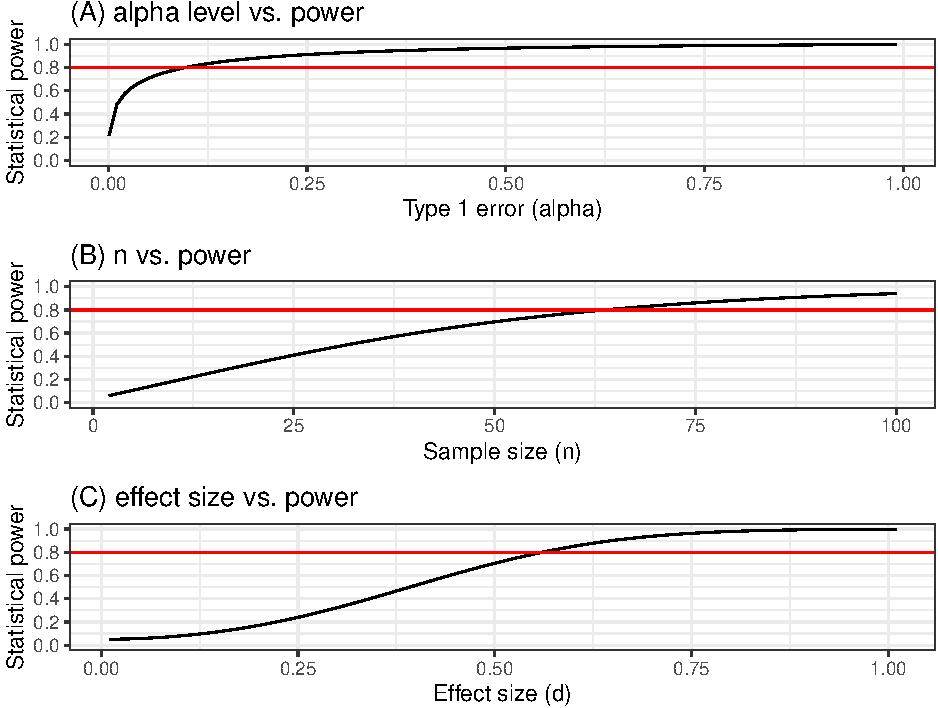
\includegraphics{code_power_analysis_short_files/figure-latex/unnamed-chunk-2-1.pdf}

\hypertarget{figure-s1}{%
\subsubsection{Figure S1}\label{figure-s1}}

An example showing how the three parameters affect the statistical
power: (A) Type I error (\(\alpha\)), (B) Sample size (\(n\)), (C)
Magnitude of the standardized effect size (\(d\)). These figures are
simulated using \texttt{retro\_design()} function in
\texttt{retrodesign} package
{[}\protect\hyperlink{ref-gelman2014beyond}{1}{]}. See the corresponding
code chunk for detailed code.

From Figure S1A we can see that when an experiment commits a higher Type
1 error (which we do not want), it is easier to achieve a desired
statistical power (i.e., Cohen's recommendation: 80\% power). Increasing
sample size (\(n\)) and magnitude of standardized effect size are
effective ways to increase the statistical power of a given experiment
(Figure S1B and S1C).

\hypertarget{estimating-sample-sizes-in-the-ficticious-experiment}{%
\subsection{Estimating sample sizes in the `ficticious'
experiment}\label{estimating-sample-sizes-in-the-ficticious-experiment}}

When designing an `hypothetical' diet experiment in your grant proposal,
You choose a common significance threshold, \(\alpha\) = 0.05 and the
nominal power level of 80\%.Based on your pilot and external information
(e.g., relevant studies or a meta-analysis on maternal effect), you
assume maternal obesogenic diet will lead to a 30\% increase in males,
20\% in females and 10\% difference between the sexes. To quantify the
diet effect using a standardized effect size (i.e., \(d\)). We assumed
the followings:

control group (both male and female) - mean = 100 (arbitrary unit) and
standard deviation (sd) = 30;

male treatment group - mean = 130 and sd = 30;

female treatment group - mean = 120 and sd = 30.

Note that we assume the homogeneity of variances among groups (i.e.~sd =
30).

\begin{Shaded}
\begin{Highlighting}[]
\DocumentationTok{\#\# scenario 1: large effects}

\DocumentationTok{\#\#\# set up an independent design}
\NormalTok{design }\OtherTok{\textless{}{-}} \FunctionTok{ANOVA\_design}\NormalTok{(}
  \AttributeTok{design =} \StringTok{"2b*2b"}\NormalTok{, }\CommentTok{\# independent design, which means no correlation}
  \AttributeTok{n =}\DecValTok{290}\NormalTok{, }\CommentTok{\# the sample size in each group for testing sex difference}
  \AttributeTok{mu =} \FunctionTok{c}\NormalTok{(}\DecValTok{130}\NormalTok{, }\DecValTok{120}\NormalTok{, }\DecValTok{100}\NormalTok{, }\DecValTok{100}\NormalTok{), }
  \AttributeTok{sd =} \DecValTok{30}\NormalTok{,}
  \AttributeTok{labelnames =} \FunctionTok{c}\NormalTok{(}\StringTok{"diet"}\NormalTok{, }\StringTok{"obesogenic "}\NormalTok{, }\StringTok{"control "}\NormalTok{, }\StringTok{"sex"}\NormalTok{, }\StringTok{"male"}\NormalTok{, }\StringTok{"female"}\NormalTok{),}
  \AttributeTok{plot =} \ConstantTok{FALSE}\NormalTok{)}

\NormalTok{meanplot\_largeES }\OtherTok{\textless{}{-}}\NormalTok{ design}\SpecialCharTok{$}\NormalTok{meansplot }\SpecialCharTok{+} \FunctionTok{labs}\NormalTok{(}\AttributeTok{x =} \StringTok{"Groups"}\NormalTok{, }\AttributeTok{y =} \StringTok{"Mean"}\NormalTok{, }\AttributeTok{title =} \StringTok{"Surprisingly large effects"}\NormalTok{)}
\NormalTok{Figure\_S2 }\OtherTok{\textless{}{-}}\NormalTok{ meanplot\_largeES}
\NormalTok{Figure\_S2}
\end{Highlighting}
\end{Shaded}

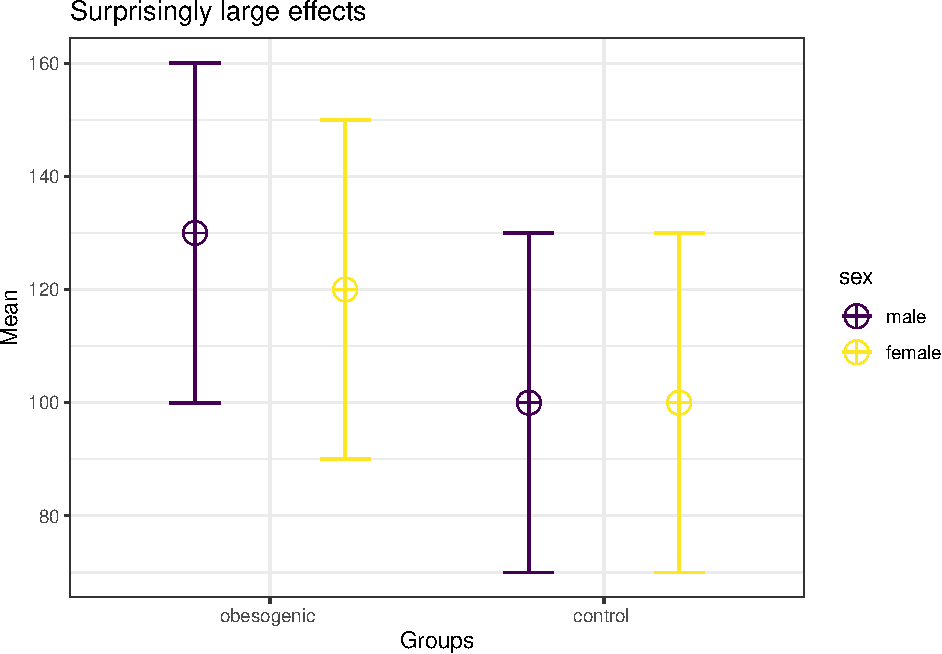
\includegraphics{code_power_analysis_short_files/figure-latex/unnamed-chunk-3-1.pdf}

\hypertarget{figure-s2}{%
\subsubsection{Figure S2}\label{figure-s2}}

Visualization of the assumed means and standard deviation (sd) of each
group. Error bars represent sd.

Using these means and sds, we have the following standardized mean
difference \(d\), corresponding \% differences:

\begin{enumerate}
\def\labelenumi{(\arabic{enumi})}
\item
  1.0, corresponding to 30\% increase of memory in males after
  intervention by diet;
\item
  0.67, corresponding to 20\% increase of memory in females after
  intervention by diet;
\item
  0.33, corresponding to sex difference or interaction between diet and
  sex.
\end{enumerate}

You are planning to use a typical two-sample t-test to examine the
statistical significance of the diet effect in males and females. Then
you can approximate sample size required for each group using the
following formula {[}\protect\hyperlink{ref-lehr1992sixteen}{2}{]}:

\[
n = \text{16} \frac{Var[θ]} {E[θ]^2} = \text{16} \frac{1} {d^2}
\] However, for the last effect (interaction effect), this requires
comparing 4 groups so that this formula does not work. Yet you can still
use this formula by replacing 16 with 32 as interaction involves four
groups rather than two.

In the following section, we use our custom function (based on the above
formula) and one existing R package \texttt{pwr} to estimate the sample
size used in your proposed experiment with different scenarios (sample
size mentioned in the fictitious story in the main text). We also
validate the sample size estimates using another package
\texttt{Superpower}.

\begin{Shaded}
\begin{Highlighting}[]
\DocumentationTok{\#\#\#\#\#\#\#\#\#\#\#\#\#\#\#\#\#\#\# power calculation}

\CommentTok{\# 2 independent group situation (assumed)}

\CommentTok{\# female control: mean = 100, sd = 30 female experiment: mean = 120, sd = 30}
\CommentTok{\# male control: mean = 100, sd = 30 male experiment: mean = 130, sd = 30}

\CommentTok{\# to meet the assumption of homogeneity of variance, both treatment and control}
\CommentTok{\# groups share a common sd. In such a case, the pooled sd also equals 30.}
\CommentTok{\# Otherwise, this critical assumption would be violated and you need to get}
\CommentTok{\# weighed average via sd\^{}2 (variance).}

\CommentTok{\# cohen\textquotesingle{}s d female}
\NormalTok{(}\DecValTok{120} \SpecialCharTok{{-}} \DecValTok{100}\NormalTok{)}\SpecialCharTok{/}\DecValTok{30}

\CommentTok{\# conhen\textquotesingle{}s d male}
\NormalTok{(}\DecValTok{130} \SpecialCharTok{{-}} \DecValTok{100}\NormalTok{)}\SpecialCharTok{/}\DecValTok{30}

\CommentTok{\# cohen\textquotesingle{}s d sex difference sex difference}
\NormalTok{((}\DecValTok{130} \SpecialCharTok{{-}} \DecValTok{100}\NormalTok{) }\SpecialCharTok{{-}}\NormalTok{ (}\DecValTok{120} \SpecialCharTok{{-}} \DecValTok{100}\NormalTok{))}\SpecialCharTok{/}\DecValTok{30}


\CommentTok{\# the first set (surprising large effects)}

\DocumentationTok{\#\# male treatment effect}
\FunctionTok{pwr.t.test}\NormalTok{(}\AttributeTok{d =} \DecValTok{1}\NormalTok{, }\AttributeTok{sig.level =} \FloatTok{0.05}\NormalTok{, }\AttributeTok{power =} \FloatTok{0.8}\NormalTok{, }\AttributeTok{type =} \StringTok{"two.sample"}\NormalTok{, }\AttributeTok{alternative =} \StringTok{"two.sided"}\NormalTok{)  }\CommentTok{\# }
\NormalTok{pwr\_independent\_m\_d1 }\OtherTok{\textless{}{-}} \FunctionTok{short\_cut}\NormalTok{(}\AttributeTok{d =} \DecValTok{1}\NormalTok{, }\AttributeTok{method =} \StringTok{"normal"}\NormalTok{)  }\CommentTok{\# our result from our custom function is very close to the pwr.t.test() function}


\DocumentationTok{\#\# female treatment effect}
\FunctionTok{pwr.t.test}\NormalTok{(}\AttributeTok{d =} \FloatTok{0.67}\NormalTok{, }\AttributeTok{sig.level =} \FloatTok{0.05}\NormalTok{, }\AttributeTok{power =} \FloatTok{0.8}\NormalTok{, }\AttributeTok{type =} \StringTok{"two.sample"}\NormalTok{, }\AttributeTok{alternative =} \StringTok{"two.sided"}\NormalTok{)}
\NormalTok{pwr\_independent\_f\_d0}\FloatTok{.67} \OtherTok{\textless{}{-}} \FunctionTok{short\_cut}\NormalTok{(}\AttributeTok{d =} \FloatTok{0.67}\NormalTok{, }\AttributeTok{method =} \StringTok{"normal"}\NormalTok{)}

\CommentTok{\# sex difference, e.g., interactive effect}
\FunctionTok{pwr.t.test}\NormalTok{(}\AttributeTok{d =} \FloatTok{0.33}\NormalTok{, }\AttributeTok{sig.level =} \FloatTok{0.05}\NormalTok{, }\AttributeTok{power =} \FloatTok{0.8}\NormalTok{, }\AttributeTok{type =} \StringTok{"two.sample"}\NormalTok{, }\AttributeTok{alternative =} \StringTok{"two.sided"}\NormalTok{)  }\CommentTok{\# INCORRECT!! Because interaction effect involves four groups rather than two groups. See details in the main text}
\NormalTok{pwr\_independent\_i\_d0}\FloatTok{.33} \OtherTok{\textless{}{-}} \FunctionTok{short\_cut}\NormalTok{(}\AttributeTok{d =} \FloatTok{0.33}\NormalTok{, }\AttributeTok{method =} \StringTok{"interaction"}\NormalTok{)  }\CommentTok{\# close enough}
\end{Highlighting}
\end{Shaded}

\hypertarget{sample-size-to-detect-presumed-effects-in-an-independent-experimental-design}{%
\subsubsection{Sample size to detect `presumed' effects in an
independent experimental
design}\label{sample-size-to-detect-presumed-effects-in-an-independent-experimental-design}}

To meet the statistical assumption of data independence of the
statistical method (i.e., ANOVA), you can only sample one male and one
female pup from one dam/mother when performing a memory assay (e.g.,
Morris water maze or fear conditioning). Then you can estimate the
sample size using the above formula or using the following syntax (see
code chunk for the explanation of each argument):

\hypertarget{refs}{}
\begin{CSLReferences}{0}{0}
\leavevmode\vadjust pre{\hypertarget{ref-gelman2014beyond}{}}%
\CSLLeftMargin{1. }
\CSLRightInline{Gelman A, Carlin J. Beyond power calculations: Assessing
type s (sign) and type m (magnitude) errors. Perspectives on
Psychological Science. 2014;9: 641--651. }

\leavevmode\vadjust pre{\hypertarget{ref-lehr1992sixteen}{}}%
\CSLLeftMargin{2. }
\CSLRightInline{Lehr R. Sixteen s-squared over d-squared: A relation for
crude sample size estimates. Statistics in medicine. 1992;11:
1099--1102. }

\end{CSLReferences}

\end{document}
